\chapter{Estado de la Cuestión}
\label{cap:estadoDeLaCuestion}



%\begin{resumen} En este capítulo se dará una idea general sobre los Sistemas Aumentativos y Alternativos de Comunicación (Sección \ref{cap3:sec:saac}) y las características de los pictogramas y los distintos sistemas pictográficos que existen (Sección \ref{cap3:sec:pictogramas}). Finalmente, se verán distintas herramientas con las que se construyen tableros de pictogramas (Sección \ref{cap3:sec:editor-tableros} ).

%\end{resumen}

Actualmente convivimos con multitud de personas pero todas cuentan con la misma facilidad para comunicarse, ya sea por discapacidad física, intelectual o sensorial. Para facilitar la comunicación de este colectivo, se utilizan otros sistemas alternativos que facilitan la comunicación.

\section{Sistemas Aumentativos y Alternativos de Comunicación}
\label{cap3:sec:saac}
Los Sistemas Aumentativos y Alternativos de Comunicación\footnote{\url{https://www.logopeda-madrid.es/tratamientos-logopedia/otros-sistemas-de-comunicacion.php}} (\textit{SAAC}) son sistemas de comunicación alternativos al lenguaje oral. Son considerados aumentativos a todos aquellos sistemas que complementan o aumentan el lenguaje oral cuando éste no basta para mantener una comunicación eficaz, y alternativos si reemplaza el lenguaje oral cuando este fuera incomprensible. 

En función de la necesidad de uso de recursos comunicativos, pueden distinguirse dos tipos:

\begin{itemize}
	\item \textbf{Sistemas sin ayuda}: permiten cambiar información entre personas sin utilizar ningún recurso externo para establecer una comunicación, únicamente usan su propio cuerpo. En los sistemas sin ayuda podemos observar dos tipos de grupos: los métodos gestuales como lengua de signos y los métodos oralistas como la lectura labiofacial, ambos utilizados por personas sordas.
	
	\item \textbf{Sistemas con ayuda}: las personas con dificultades de comunicación utilizan recursos externos para establecer una comunicación, las cuales permiten hacer preguntas, expresar sentimientos o realizar peticiones. Los recursos pueden ser símbolos, pictogramas o dibujos y pueden encontrarse en soportes analógicos, como cartulinas o tableros, o bien mediante soportes digitales, como aplicaciones para móvil.
\end{itemize}

En este trabajo nos enfocaremos en los sistemas con ayuda, concretamente en los pictogramas. Comúnmente utilizados por personas con discapacidades intelectuales o físicas.


\section{Pictogramas}
\label{cap3:sec:pictogramas}
Los pictogramas son imágenes o símbolos de rápida comprensión que expresan acciones, objetos, emociones, etc. Un conjunto de pictogramas en un cierto orden pueden representar una oración. Todos ellos deben cumplir las siguientes características\footnote{\url{http://aularagon.catedu.es/materialesaularagon2013/arasaac/ZIPs/Modulo_1/contenidos.html}}:
\begin{enumerate}
	\item \textbf{Referencialidad}: relación del pictograma con el referente.
	\item \textbf{Ítems gráficos}: imágenes que representen de manera sencilla aquello que se toma como modelo.
	\item \textbf{Comprensión}: deben ser fácilmente entendibles independientemente de la formación, idioma o discapacidad.
	\item \textbf{Legibilidad}: deben mantener una coherencia visual entre pictogramas.
	\item \textbf{Sencillez}: mostrar únicamente los elementos relevantes sin elementos distractores o adornos insignificantes.
\end{enumerate}


 
Existen numerosos sistemas pictográficos. A continuación hablaremos de algunos de los más relevantes.

\subsection{Sistema Pictográfico de Comunicación - SPC}
\label{cap3:sec:spc}
El Sistema Pictográfico de Comunicación\footnote{\url{https://www.uv.es/bellochc/logopedia/NRTLogo8.wiki?8}} (\textit{SPC}) fue creado en 1981 por Roxana Mayer Johnson, con la intención de facilitar la comunicación a quienes tienen un nivel de lenguaje expresivo simple o vocabulario limitado. Gracias a la diferenciación por colores, facilita la comprensión de la estructura sintáctica. Actualmente cuenta con más de 3.000 iconos. Está organizado por seis colores según su función gramatical, como podemos ver en la Figura \ref{fig:spccolores}.

\begin{itemize}
	\item \textbf{Personas} (Amarillo): representan a familiares y pronombres. Ejemplo: mamá, familia,  yo, ellos.
	\item \textbf{Verbos} (Verde): representan acciones. Ejemplo: abrir, agarrar, comer, ir.
	\item \textbf{Descriptivos} (Azul): representan descripciones, adjetivos y adverbios. Ejemplo: bonito, triste, vacío, lleno.
	\item \textbf{Nombre} (Naranja): representan objetos u otros elementos que no aparecen en otra categoría. Ejemplo: gato, almohada o casa.
	\item \textbf{Miscelánea} (Blanco): representa números, letras y colores
	\item \textbf{Social} (Rosa): vocabulario relacionado con relaciones sociales. Ejemplo: buenos días, sí, gracias, no lo sé.
	
\end{itemize}

% TODO: \usepackage{graphicx} required
\begin{figure}[h!]
	\centering
	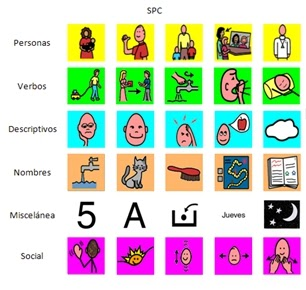
\includegraphics[width=0.8\linewidth]{Imagenes/Bitmap/SPCcolores}
	\caption{Ejemplo de categorías en SPC.}
	\label{fig:spccolores}
\end{figure}

\subsection{Blissymbolics}
\label{cap3:sec:Blissymbolics}
Byssimbolics\footnote{\url{https://www.blissymbolics.org/index.php/about-blissymbolics}}
es un sistema de comunicación que fue usado por primera vez en 1971 para facilitar la comunicación con niños que padecían alguna discapacidad. Actualmente está compuesto por más de 5.000 símbolos o  \textit{Bliss-Words}, los cuales a su vez están compuestos por uno o más Caracteres-Bliss o  \textit{Bliss-Characters}. A pesar de que los 150 \textit{Bliss-Characters} que hay son sencillos de dibujar, requieren un periodo de aprendizaje para comprender su significado y así también el de las \textit{Bliss-Words}. En la Figura \ref{fig:blisscharacters} vemos algunos \textit{Bliss-Characters} con su significado. \\
% TODO: \usepackage{graphicx} required

\begin{figure}[h!]
	\centering
	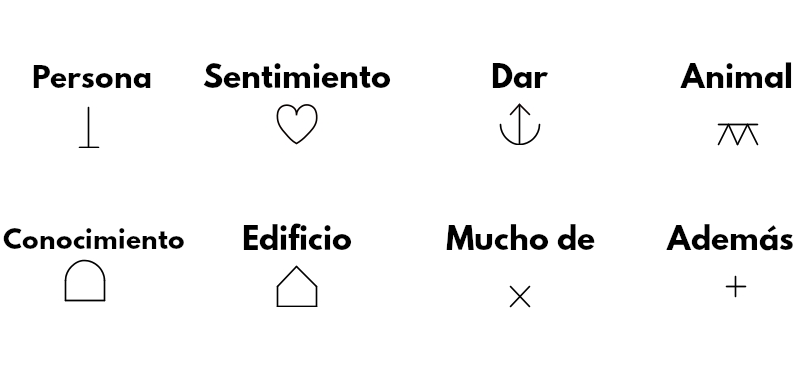
\includegraphics[width=0.8\linewidth]{Imagenes/Bitmap/BlissCharacters}
	\caption[Ejemplo de Bliss-Characters]{Ejemplo de Bliss-Characters.}
	\label{fig:blisscharacters}
\end{figure}
Una vez comprendidos los \textit{Bliss-Characters}, en la Figura \ref{fig:blissword} vemos cómo se han combinado para generar \textit{Bliss-Words}. Destacar que el orden, el tamaño o la posición de los los Bliss-Characters puede alterar su significado. Adicionalmente pueden estar agrupados usando los mismos colores vistos en SPC.

% TODO: \usepackage{graphicx} required
\begin{figure}[h!]
	\centering
	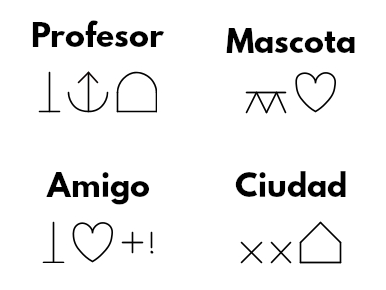
\includegraphics[width=0.4\linewidth]{Imagenes/Bitmap/BlissWord}
	\caption[Ejemplo de Bliss-Words]{Ejemplo de Bliss-Words.}
	\label{fig:blissword}
\end{figure}



\subsection{Sclera}
La principal característica de Sclera\footnote{\url{https://www.sclera.be/en/picto/overview}} frente a otros sistemas pictográficos es que sus pictogramas son menos coloridos, pero cuentan con pictogramas más avanzados en cuanto a las acciones representadas. Un ejemplo de ello se puede ver en la Figura \ref{fig:sclera} donde la acción de pedir atención se puede realizar de dos maneras posibles. Cuenta con un total de 11.497 pictogramas en español. En la actualidad el desarrollo de Sclera está paralizado desde 2015.



% TODO: \usepackage{graphicx} required
\begin{figure}[h!]
	\centering
	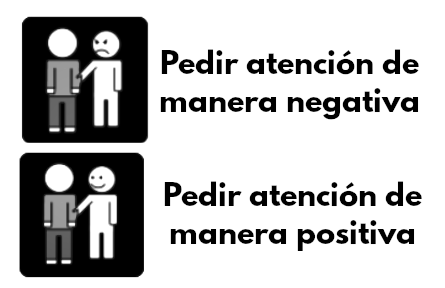
\includegraphics[scale=0.4]{Imagenes/Bitmap/Sclera}
	\caption{Ejemplo de acciones en Sclera.}
	\label{fig:sclera}
\end{figure}


\subsection{Mulberry Symbols}
\label{cap3:sec:mulberry}
Mulberry Symbols\footnote{\url{https://mulberrysymbols.org/}} se creó con el propósito de ser un sistema pictográfico orientado a adultos, ya que un gran porcentaje de dichos sistemas estaban pensados principalmente para niños y dificultaban la comunicación por falta de pictogramas. Como se observa en la Figura \ref{fig:mulberry} podemos ver ejemplos de pictogramas enfocados a adultos como cerveza o fumar.

% TODO: \usepackage{graphicx} required
\begin{figure}[h!]
	\centering
	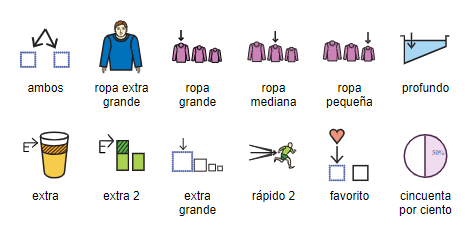
\includegraphics[scale=0.2]{Imagenes/Bitmap/Mulberry}
	\caption{Ejemplo de pictogramas de Mulberry.}
	\label{fig:mulberry}
\end{figure}

Todos los pictogramas pueden descargarse gratuitamente desde su página web en formato ZIP, y las imágenes se encuentran en formato SVG o formato CSV donde están categorizados según su nombre y categoría. 
Los pictogramas de Mulberry cuentan con 118 categorías incluyendo sustantivos, pronombres y verbos sumando un total de 3.436 pictogramas. A diferencia de otros sistemas pictográficos, Mulberry sigue en activo añadiendo constantemente nuevos pictogramas. 

Los pictogramas de Mulberry son utilizados por muchas aplicaciones como BoradBuilder\footnote{\url{ https://globalsymbols.com/boardbuilder/boardsets}} (aplicación web para diseñar tableros de comunicación), Cboard\footnote{\url{https://www.cboard.io/}} (aplicación web de comunicación que usa pictogramas y conversión de texto a voz) o CommuniKate\footnote{\url{http://communikate.equalitytime.co.uk/}} (página web que ofrece tableros diseñados en Powerpoint o Impress). Una de las últimas herramientas creadas que hace uso de los pictogramas de Mulberry es la diseñada por Eliada Pampoulou y Maria Constanta de la Universidad Tecnológica de Chipre la cual usa unas plantillas imprimibles en inglés\footnote{\url{https://mulberrysymbols.org/assets/COVID19/Covid-19_AAC-EN.pdf}} o griego para ayudar a la comunicación de los pacientes con la COVID-19 que tienen dificultades para comunicarse.






\subsection{Minspeak}
\label{cap3:sec:minspeak}
Minspeak\footnote{\url{http://ares.cnice.mec.es/informes/18/contenidos/94.htm}}, es un sistema de comunicación alternativo creado por Bruce Baker en 1982. Difiere con los vistos anteriormente en que el significado de los iconos no viene preestablecido sino que es acordado entre usuario y logopeda. Es por ello que cada icono acordado tenga un significado distinto según la secuenciación de iconos. Por ejemplo, en el caso de la Figura \ref{fig:minspeak} la asociación del icono casa junto a la cama en un orden podría ser interpretado como dormitorio. 

% TODO: \usepackage{graphicx} required
\begin{figure}[h!]
	\centering
	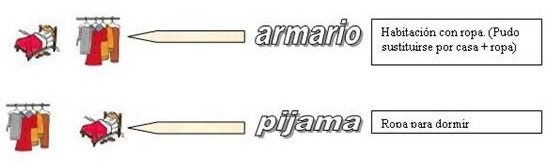
\includegraphics[width=0.9\linewidth]{Imagenes/Bitmap/Minspeak}
	\caption{Ejemplo de Minspeak.}
	\label{fig:minspeak}
\end{figure}

Como cada pictograma puede tener un significado distinto según su orden, se crearon Programas de Comunicación Minspeak (\textit{PAM}). Éstos se usan para que cuando una casilla o icono haya sido seleccionada, se activen los posibles iconos con los que pueda tener algún tipo de relación. Inicialmente se creó hardware específico (como aparece en la Figura \ref{fig:chatbox}) con 16 celdas las cuales podía generar hasta 1.024 mensajes, estos teclados evolucionaron con más celdas y combinaciones, hasta pasar a teclados digitales implementados por software como PortaVoz\footnote{\url{http://www.terapia-ocupacional.com/articulos/Portavoz_JMLedesma.shtml}}.

% TODO: \usepackage{graphicx} required
\begin{figure}[h!]
	\centering
	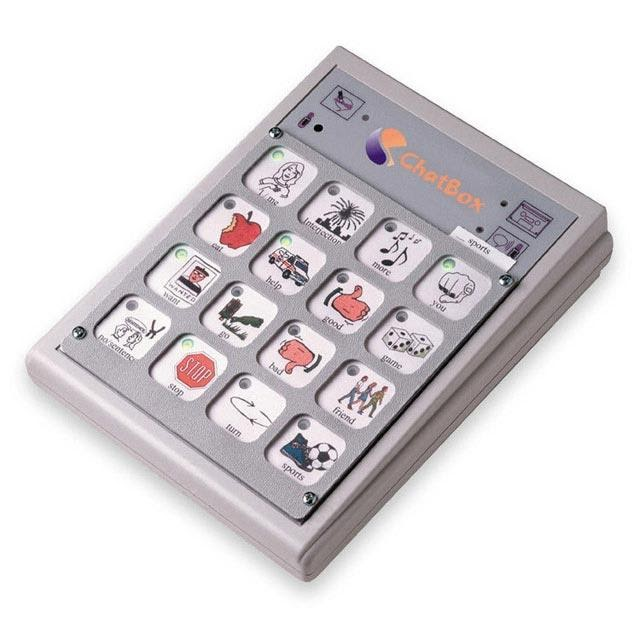
\includegraphics[width=0.4\linewidth]{Imagenes/Bitmap/ChatBox}
	\caption[ChatBox]{Panel de ChatBox}
	\label{fig:chatbox}
\end{figure}



\subsection{ARASAAC}
\label{cap3:sec:arasaac}
El portal Aragonés de Comunicación Aumentativa y Alternativa  (\textit{ARASAAC}\footnote{\url{http://www.arasaac.org/}})
 surge en 2007 gracias a la colaboración entre el personal del CATEDU, el colegio público de educación Especial Alborada y del Centro Politécnico Superior de la Universidad de Zaragoza. Su objetivo era la creación de un sistema pictográfico de libre distribución que ayudara en el ámbito de la comunicación a todas aquellas personas que lo necesitasen.
Actualmente el portal de \textit{ARASAAC} incluye fotografías, vídeos y cuenta con más de 3.9000 pictogramas tanto a color como en blanco y negro y con traducciones a 20 idiomas. También ofrece herramientas online con las que poder generar materiales como por ejemplo calendarios, tableros, creador de símbolos, etc.

A diferencia de otros sistemas pictográficos, \textit{ARASAAC} permite una gran cantidad de opciones configurables como el color de fondo, el marco o el tiempo verbal. Estas opciones se pueden ver en la Figura \ref{fig:configuarcion-arasaac} donde además de las opciones vistas, se puede modificar cambiar la posición del texto, la resolución o su posición\footnote{\url{https://arasaac.org/pictograms/es/6009/hola}}.



\begin{figure}[h!]
	\centering
	\includegraphics[width=0.7\linewidth]{Imagenes/Bitmap/Configuarción ARASAAC}
	\caption{Opciones de configuración de un pictograma.}
	\label{fig:configuarcion-arasaac}
\end{figure}



En la actualidad \textit{ARASAAC} es uno de los sistemas pictográficos más utilizados a nivel de educación especial en España. Sus pictogramas se utilizan en colegios, universidades e incluso se han creado asociaciones para facilitar su implantación. CreaTea\footnote{\url{https://www.ayudaleayudate.es/wp-content/uploads/2019/02/Dossier-Createa.pdf}} es una asociación en la Comunidad de Madrid cuyo objetivo es habilitar lugares como clínicas, restaurantes o ayuntamientos, para ayudar a la inclusión de personas con dificultades en la comunicación y concienciar a la sociedad.

También cabe destacar que \textit{ARASAAC} ha recibido varios premios por su labor y que es una herramienta utilizada en varios países por lo que la cantidad de usuarios que colaboran es muy alta. Esto queda reflejado en la cantidad de pictogramas que se publican a la plataforma por parte de colaboradores sin ánimo de lucro y dichos pictogramas están constantemente actualizándose. Un ejemplo de ellos son los pictogramas que se han publicado debido a la pandemia como por ejemplo los que podemos ver en la Figura \ref{fig:ejemplosdepictos}.


% TODO: \usepackage{graphicx} required
\begin{figure}[h!]
	\centering
	
\includegraphics[width=0.7\linewidth]{Imagenes/Bitmap/ejemplosdepictos}
	\caption{Nuevos pictogramas creados debido a la situación actual de pandemia. }
	\label{fig:ejemplosdepictos}
\end{figure}




En la Figura \ref{fig:arasaacpictos} podemos ver algunos ejemplos de pictogramas de ARASAAC en situaciones o casos más cotidianos. Destacan la manera clara y concisa en la que están representados. 

% TODO: \usepackage{graphicx} required
\begin{figure}[h!]
	\centering
	
\includegraphics[width=0.7\linewidth]{Imagenes/Bitmap/ARASAACPictos}
	\caption{Ejemplo de pictogramas más típicos de \textit{ARASAAC}.}
	\label{fig:arasaacpictos}
\end{figure}

La licencia de \textit{ARASAAC} es de tipo \textit{Creative Commons (BY-NC-SA)}, por lo que se podrá utilizar el material elaborado por ellos de cara a la implementación del Trabajo Fin de Grado. Utilizaremos sus pictogramas publicados en su página web y la API que han desarrollado para acceder a pictogramas de su base de datos.

\section{Aplicaciones basadas en pictogramas}
\label{cap3:sec:editor-tableros}

Ya hemos visto multitud de sistemas pictográficos. Pero para trabajar con ellos es necesario que sean fáciles de acceder, pues lo normal encontrar cientos de pictogramas en cada sistema pictográfico. La solución a este problema, son los tableros pictográficos. Los tableros son un área en la que se pueden colocar pictogramas, fotografías o palabras que la persona indicará para comunicarse. Pueden tener distintas funciones, como por ejemplo hacer un horario, normas, o elegir entre distintas opciones mediante pictogramas. A menudo estos tableros se realizan mediante piezas de papel recortadas, como podemos ver en la Figura \ref{fig:editorespictogramas}.

% TODO: \usepackage{graphicx} required
\begin{figure}[h!]
	\centering
	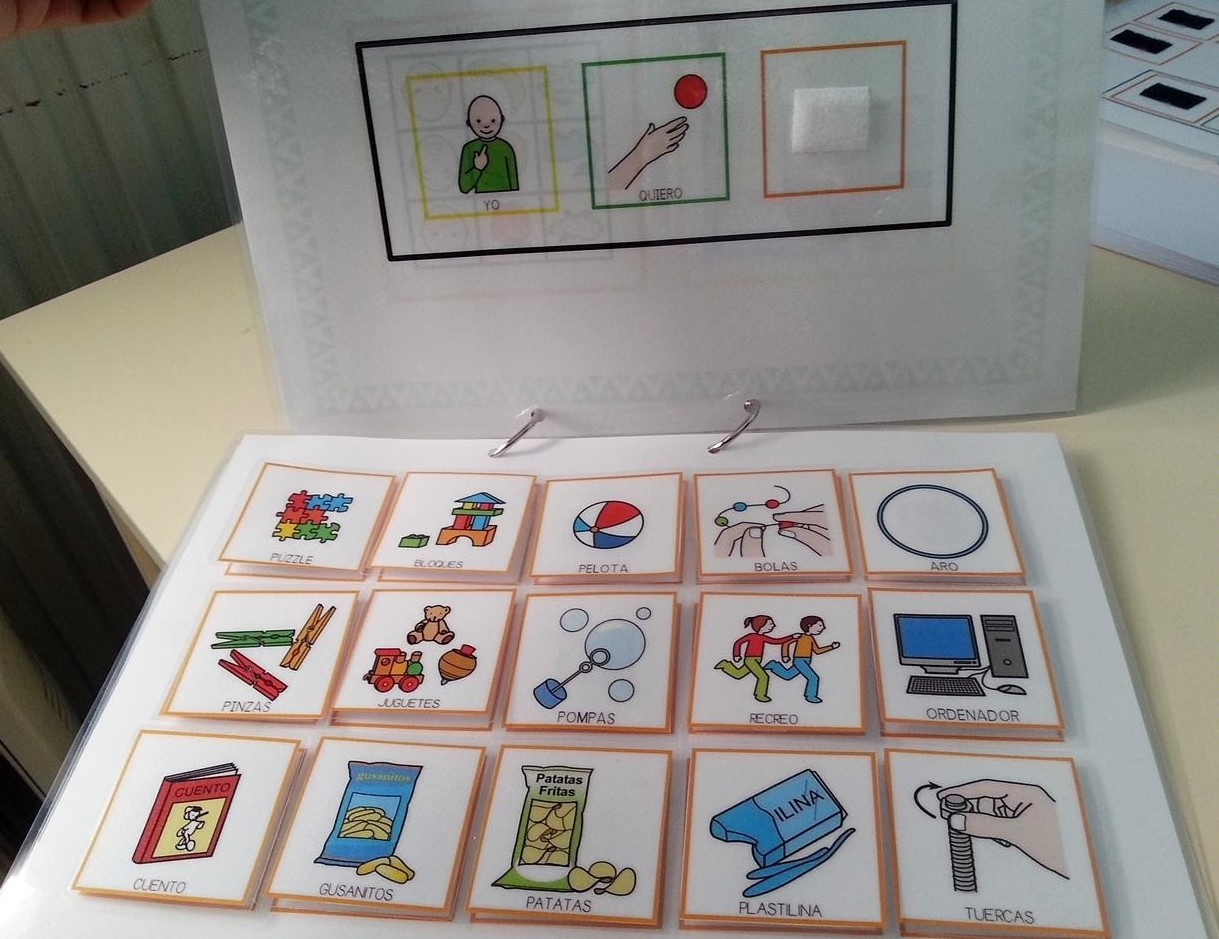
\includegraphics[width=0.7\linewidth]{Imagenes/Bitmap/EditoresPictogramas}
	\caption{Ejemplo de tablero para pictogramas en papel.}
	\label{fig:editorespictogramas}
\end{figure}

Estos tableros\footnote{\url{http://burbujadelenguaje.blogspot.com/2016/05/tablero-de-comunicacion-tea.html}} no tienen por qué limitarse a un espacio rectangular, sino que se pueden usar de maneras más creativas dependiendo de las discapacidades de la persona que lo use. Por ejemplo los \textit{ETRAN}\footnote{\url{http://psicosociosanitario.blogspot.com/2016/05/tableros-de-comunicacion.html}} (“Eye-Transfer”) son usados por gente con baja movilidad y que apuntan al pictograma con la mirada, de manera que otra persona está al otro lado del \textit{ETRAN} para ver qué pictograma está mirando como podemos ver en la Figura \ref{fig:tablero}. Otro ejemplo son los cuadernos de comunicación, que como su nombre indica son un conjunto de hojas o tableros con símbolos básicos.

% TODO: \usepackage{graphicx} required
\begin{figure}[h!]
	\centering
	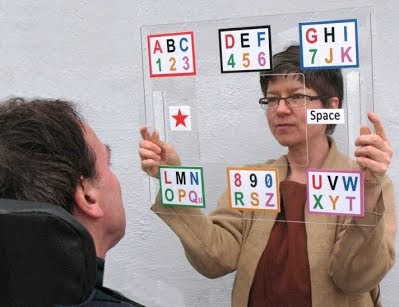
\includegraphics[width=0.7\linewidth]{Imagenes/Bitmap/Tablero}
	\caption{Uso de tablero ETRAN.}
	\label{fig:tablero}
\end{figure}

Como trabajar con piezas de papel puede resultar engorroso y a menudo poco eficiente, los tableros pictográficos han sufrido una evolución natural al medio digital, y con ello ha aparecido gran cantidad de software de edición de tableros pictográficos. Gracias a ello, las personas que usan estos nuevos sistemas ahorran mucho tiempo, como buscar pictogramas rápidamente, alinearlos perfectamente, editarlos o incluso poder compartir los tableros.


Para crear y editar tableros se han creado multitud de aplicaciones. A continuación estudiaremos algunas de sus características.



\subsection{Pictoselector}
\label{cap2:sec:pictoselector}
Pictoselector\footnote{\url{ https://www.pictoselector.eu/es/ }} una herramienta gratuita para crear agendas visuales.  Recopila más de 28.000 pictogramas provenientes de \textit{Sclera}, \textit{Mulberry}, \textit{ARASAAC}, etc. Al crear un proyecto, permite cargar una plantilla o crear una desde cero. Se puede modificar el número de filas y columnas, la posición del texto y el tamaño del borde de los pictogramas como podemos ver en la Figura \ref{fig:pictoselector-tablero} .


% TODO: \usepackage{graphicx} required
\begin{figure}[h!]
	\centering
	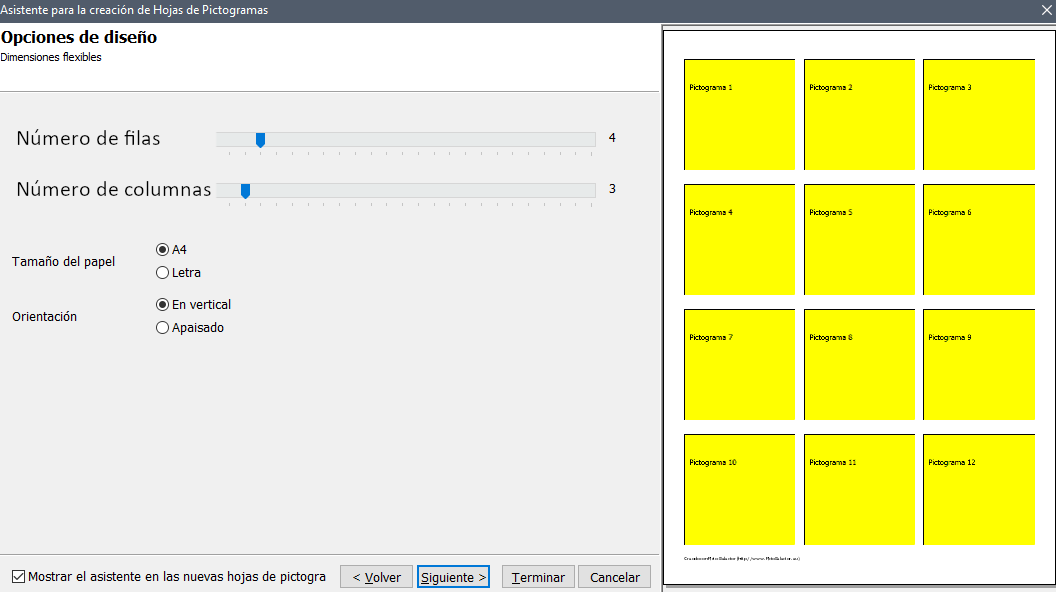
\includegraphics[width=0.7\linewidth]{Imagenes/Bitmap/Pictoselector Tablero}
	\caption{Ventana donde se edita el tamaño de la cuadrícula en el programa Pictoselector.}
	\label{fig:pictoselector-tablero}
\end{figure}


Una vez creado el tablero, podemos insertar en su cuadrícula distintos elementos, muchos de ellos en forma de pictograma. Para facilitar esta tarea, la cabecera de la aplicación contiene acceso directo a la inserción de pictogramas, como podemos ver en la Figura \ref{fig:ribbon-pictoselector}. De izquierda a derecha, existe un buscador de pictogramas que incluye la función de filtrar por juego de pictogramas como se ve en la Figura \ref{fig:editor-y-buscador-de-pictoselector}. Además permite editar ligeramente el picto ya sea coloreándolo o añadiendo un signo de pasado, presente o plural. Para el marcaje de tiempo pueden incluirse con facilidad pictogramas de reloj que marcan la hora, y de duración que marcan un intervalo de tiempo. Adicionalmente se puede importar imágenes propias, códigos QR, texto o emoticonos.
% TODO: \usepackage{graphicx} required
\begin{figure}[h!]
	\centering
	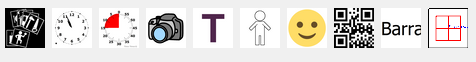
\includegraphics[width=0.9\linewidth]{Imagenes/Bitmap/Ribbon Pictoselector}
	\caption{Barra de inserción de pictogramas.}
	\label{fig:ribbon-pictoselector}
\end{figure}

% TODO: \usepackage{graphicx} required
\begin{figure}[h!]
	\centering
	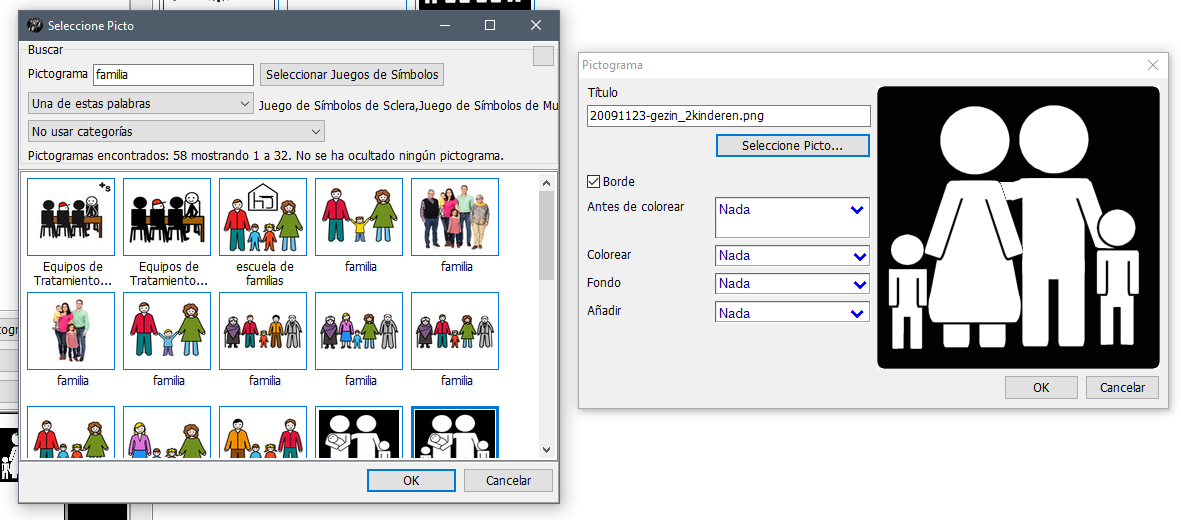
\includegraphics[width=1\linewidth]{Imagenes/Bitmap/Editor y buscador de pictoselector}
	\caption{Buscador y editor de Pictogramas.}
	\label{fig:editor-y-buscador-de-pictoselector}
\end{figure}

A pesar de ser una herramienta muy completa respecto a búsqueda y edición de pictogramas, la colocación de éstos está limitada a una cuadrícula. Por ello, no se pueden colocar pictogramas de distintos tamaños con facilidad o en posiciones intermedias.

\subsection{Editor ARASAAC}
La página web de ARASAAC\footnote{\url{http://www.arasaac.org/herramientas.php}} cuenta con diversas herramientas online que se pueden usar para generar materiales:
\begin{itemize}
\item \textbf{Creador de animaciones}: genera una animación con los pictogramas que queramos en formato GIF o SWF. También permite configurar el intervalo entre los pictogramas y el número de repeticiones que hará.

\item \textbf{Creador de símbolos}: permite la personalización de pictogramas donde podremos cambiar el nombre del pictograma, poner su traducción, modificar la fuente del texto, poner un marco, ampliar la imagen y cambiar el fondo.

\item \textbf{Generador de frases}: consta de un total de tres pasos a seguir. El primero de ellos consiste en seleccionar las palabras que queramos traducir a pictogramas. El segundo paso nos mostrará todos los pictogramas asociados para cada palabra introducida y deberemos seleccionar el que más nos guste. Y en el tercer paso aparecerán todos los pictogramas colocados en una tabla en la cual podremos añadir un marco, insertar el nombre de los pictogramas y hacer más grande la tabla resultante. En la Figura \ref{fig:frase-arasaac} podemos ver la traducción de la frase: "Me gustan los helados".


% TODO: \usepackage{graphicx} required
\begin{figure}[h!]
	\centering
	
\includegraphics[width=0.7\linewidth]{Imagenes/Bitmap/Frase ARASAAC}
	\caption{Ejemplo con el generador de frases.}
	\label{fig:frase-arasaac}
\end{figure}


\item \textbf{Generador de horarios}: genera un horario donde previamente tendremos que configurar una plantilla con los días, horas, el formato (horizontal o vertical), idioma, bordes del horario, texto para cada día y hora, y la opción de insertar un pictograma en función de su día y hora. En la Figura \ref{fig:horarioarasaac} vemos un horario generado por esta herramienta en el que se especifica para cada día y hora una acción a realizar.

% TODO: \usepackage{graphicx} required
\begin{figure}[h!]
	\centering
	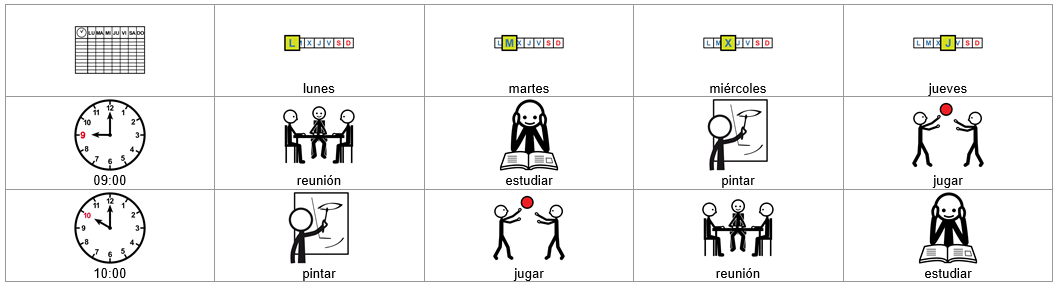
\includegraphics[width=0.9\linewidth]{Imagenes/Bitmap/HorarioARASAAC}
	\caption{Ejemplo con el generador de horarios.}
	\label{fig:horarioarasaac}
\end{figure}


\item \textbf{Generador de calendarios}: genera un calendario donde tendremos que especificar el mes, año e idioma deseado. Al igual que en el generador de horarios, permite la opción de modificar el texto, colores, bordes y la posibilidad de poner un pictograma para cada día del mes. En la Figura \ref{fig:calendarioarasaac} vemos el calendario generado para el mes de Noviembre de 2020

% TODO: \usepackage{graphicx} required
\begin{figure}[h!]
	\centering
	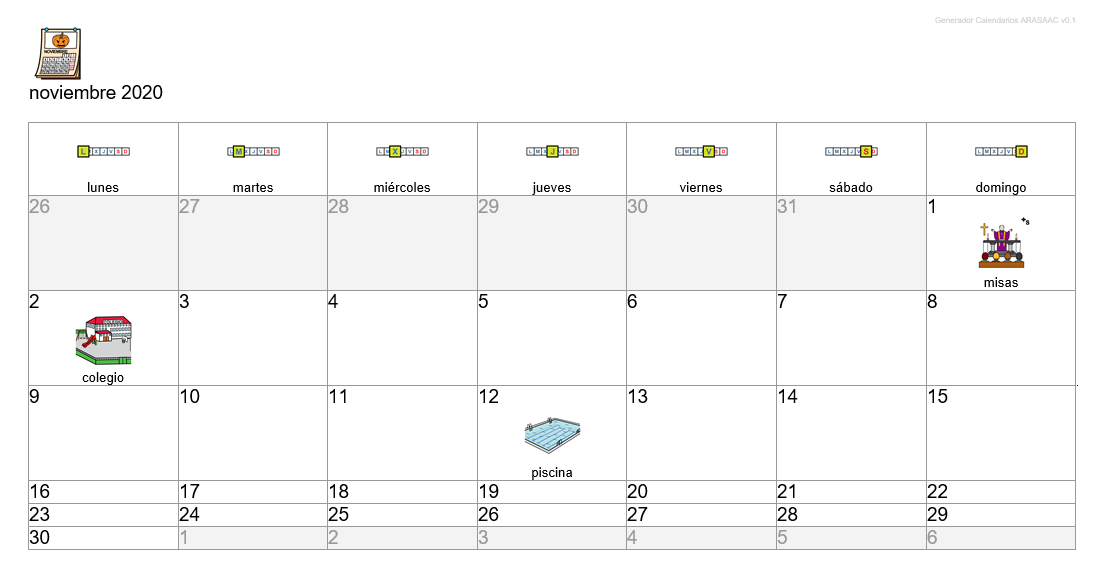
\includegraphics[width=0.7\linewidth]{Imagenes/Bitmap/calendarioARASAAC}
	\caption{Ejemplo con el generador de calendarios.}
	\label{fig:calendarioarasaac}
\end{figure}


\item \textbf{Generador de tableros}: crea un tablero con el número de filas y columnas deseado donde para cada casilla podremos insertar un pictograma. Al igual que en otras herramientas permite la modificación de colores, bordes y  texto del tablero.

\item \textbf{Creador de juegos}: genera una plantilla en formato .rtf para poder jugar al bingo, oca, dominós y dominós encadenados con los pictogramas que deseemos. En la Figura \ref{fig:juegoarasaac} vemos la creación de un tablero para jugar al bingo.

% TODO: \usepackage{graphicx} required
\begin{figure}[h!]
	\centering
	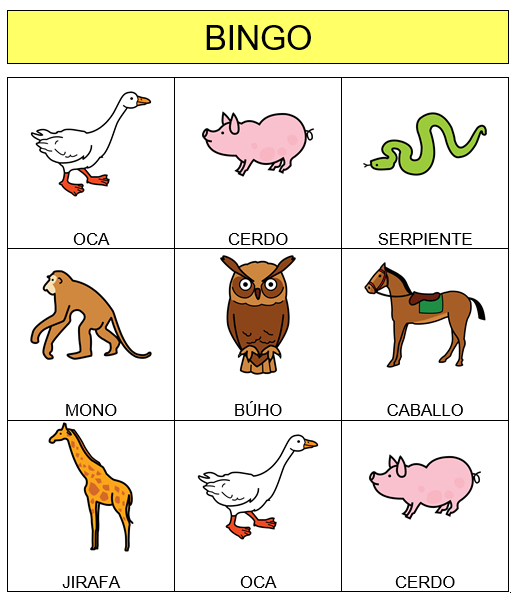
\includegraphics[width=0.7\linewidth]{Imagenes/Bitmap/juegoARASAAC}
	\caption{Ejemplo con el generador de juegos.}
	\label{fig:juegoarasaac}
\end{figure}



\end{itemize}

\subsection{Piktoplus}
\label{cap2:pkplus}
Piktoplus\footnote{\url{http://www.aulautista.com/2013/12/05/piktoplus-un-comunicador-android-muy-especial/}} es una aplicación para dispositivos Android que tiene como particularidad la creación de un avatar tridimensional personalizable. Dicho avatar será usado en los tableros pictográficos pues será quien protagonice las acciones. Permite registrar múltiples usuarios, cada uno con su propio avatar. Otra particularidad de Piktoplus son los sub-tableros\footnote{\url{https://fatimamikel.wordpress.com/2014/04/17/piktoplus-2/ }}. Por ejemplo, en la Figura \ref{fig:piktoplus1}  podemos ver un tablero con dos pictogramas: “Estoy” y “Me duele”.


% TODO: \usepackage{graphicx} required
\begin{figure}[h!]
	\centering
	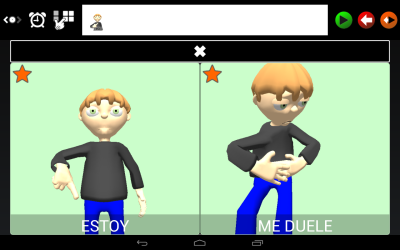
\includegraphics[width=0.5\linewidth]{Imagenes/Bitmap/Piktoplus1}
	\caption[Pictoplus tablero]{Ejemplo de tablero en Piktoplus}
	\label{fig:piktoplus1}
\end{figure}

La función de dicho sub-tablero es la de mostrar pictogramas relacionados con el picto seleccionado para formar una frase de manera más natural. Por ejemplo, si seleccionamos el pictograma de “\textit{Estoy}” como en la Figura  \ref{fig:piktoplus2}, aparecería el sub-tablero con cuatro posibles pictogramas relacionados. En este caso aparecen relacionados con el estado anímico, facilitando la creación de la frase “\textit{Estoy + Contento}”. 




% TODO: \usepackage{graphicx} required
\begin{figure}[h!]
	\centering
	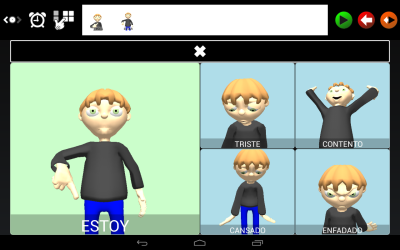
\includegraphics[width=0.5\linewidth]{Imagenes/Bitmap/Piktoplus2}
	\caption[Subtablero Piktoplus]{Subtablero en Piktoplus}
	\label{fig:piktoplus2}
\end{figure}


Respecto a la creación y edición de tableros, se trata de una cuadrícula sobre la cual se colocan los pictogramas, además permite aumentar el tamaño de los pictos. Por ejemplo “Estoy” ocupa cuatro celdas más que “Contento”. 

Actualmente esta aplicación no está disponible para descargar en tiendas de aplicaciones  habituales y su desarrollo ha cesado desde 2018. Aunque no esté disponible, plantea una idea muy interesante como la posibilidad de desplegar un sub-tablero a partir de un pictograma para mostrar pictogramas relacionados entre ellos.

\subsection{Pictar}
Pictar\footnote{\url{http://hypatia.fdi.ucm.es/pictar/}} es una aplicación web desarrollada por Alejandro Martín Guerrero de la Universidad Complutense de Madrid como Trabajo de Fin de Máster \citep{TFMPictar}. El propósito de Pictar es poder tener una aplicación web accesible desde cualquier dispositivo con conexión a internet para facilitar la comunicación a personas con TEA.

Pictar ofrece tres herramientas en su página web:
\begin{itemize}
	\item \textbf{Traducir frase}: permite generar una secuencia de pictogramas asociados a una frase o texto introducido por el usuario. Ofrece la posibilidad, tras haber generado la secuencia de pictogramas, de poder cambiarlos por otros pictogramas del mismo significado mediante unas flechas que se encuentran tanto encima como debajo de cada pictograma. También incluye un icono que tiene como finalidad copiar la secuencia de pictogramas generados al tablero (ver la Figura \ref{fig:traducirfrase}).
	
	% TODO: \usepackage{graphicx} required
	\begin{figure}[h!]
		\centering
		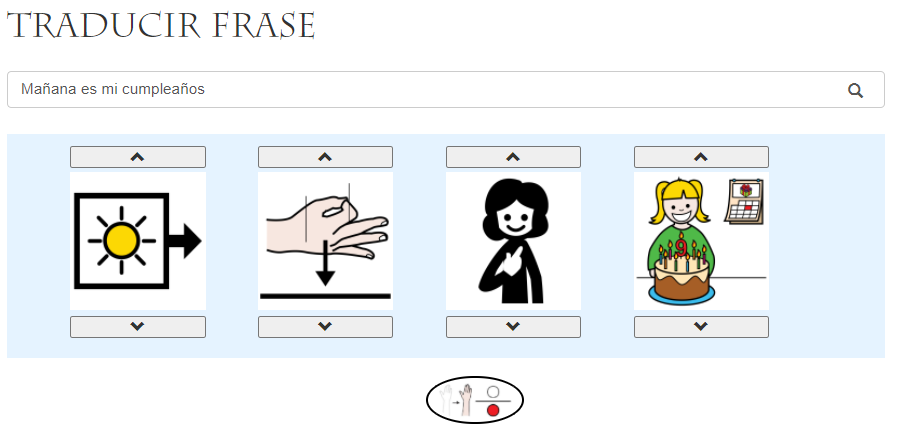
\includegraphics[width=0.7\linewidth]{Imagenes/Bitmap/TraducirFrase}
		\caption{Funcionalidad en la aplicación Pictar de traducir frase.}
		\label{fig:traducirfrase}
	\end{figure}

	\item \textbf{Buscador}: al introducir una palabra en el campo de búsqueda nos mostrará todos aquellos pictogramas con un significado igual o similar a la palabra introducida. Podemos ver un ejemplo de ello en la Figura \ref{fig:buscador}. El buscador ofrece la posibilidad de poder arrastrar los pictogramas para insertarlos al tablero que se muestra en la Figura \ref{fig:editor}.
	
	% TODO: \usepackage{graphicx} required
	\begin{figure}[h!]
		\centering
		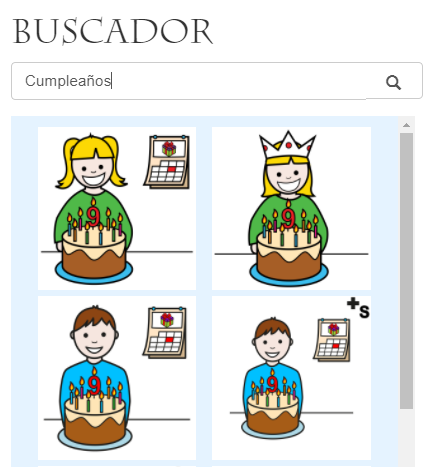
\includegraphics[width=0.5\linewidth]{Imagenes/Bitmap/buscador}
		\caption{Funcionalidad en la aplicación Pictar de buscador.}
		\label{fig:buscador}
	\end{figure}
	
	
	\item \textbf{Editor}: permite generar un tablero de pictogramas en el que deberemos seleccionar cuantos elementos va a tener en total y el número de columnas en los que se divide. Para añadir pictogramas al tablero tenemos dos opciones: la primera de ella es copiar la secuencia generada al traducir una frase a pictogramas y la segunda buscar un pictograma en el buscador para poder arrastrar el pictograma deseado al tablero. Por cada pictograma insertado en el tablero tendremos dos opciones debajo de éste situadas en las esquinas inferiores izquierda y derecha que permiten eliminar o dejar la casilla en blanco. El editor ofrece la posibilidad de añadir el nombre a cada pictograma, poner todos los pictogramas a color o blanco y negro y exportar o importar el tablero. Todas estas características se pueden observar en la Figura \ref{fig:editor}.
	
	% TODO: \usepackage{graphicx} required
	\begin{figure}[h!]
		\centering
		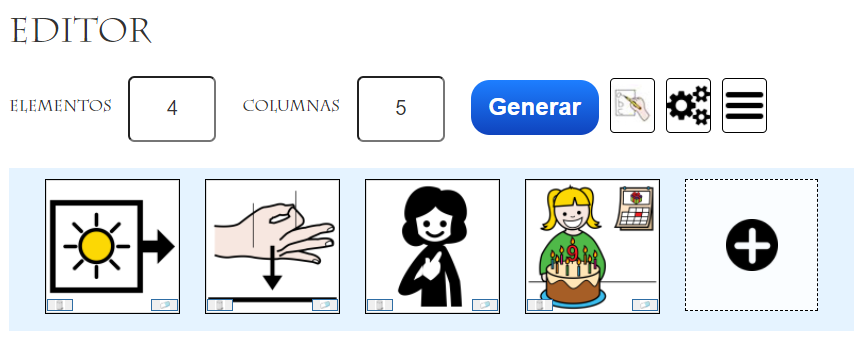
\includegraphics[width=0.7\linewidth]{Imagenes/Bitmap/editor}
		\caption{Funcionalidad en la aplicación Pictar de editor.}
		\label{fig:editor}
	\end{figure}
	
	
\end{itemize}


\subsection{PicTableros}
\label{cap2:pictableros}

PicTableros\footnote{\url{https://holstein.fdi.ucm.es/picto-tableros/}} es una aplicación web desarrollada por Carmen López Gonzalo de la Universidad Complutense de Madrid en el Grado de Ingeniería Informática como Trabajo de Fin de Grado \citep{TFGPicTableros}. PicTableros tiene como objetivo ayudar a la comunicación de personas con discapacidades cognitivas y poder realizar de una forma ágil plantillas y tableros. 
La aplicación tiene dos partes diferenciadas:
\begin{itemize}
	\item \textbf{Plantillas}: en la sección de plantillas se permite seleccionar tres modalidades: públicas, crear nuevas y privadas. En el apartado de públicas permite elegir diferentes plantillas ya creadas que las podremos usar como tableros, (ver Figura \ref{fig:pictablerosplantilla}). 
	En el apartado de crear nuevas nos permitirá añadir en la plantilla áreas para insertar pictogramas, texto y formas como triángulos, estrellas, flechas, etc. Y por último en la sección  de privadas podremos exportar o importar plantillas que tengamos creadas en nuestro equipo.
	
	% TODO: \usepackage{graphicx} required
	\begin{figure}[h!]
		\centering
		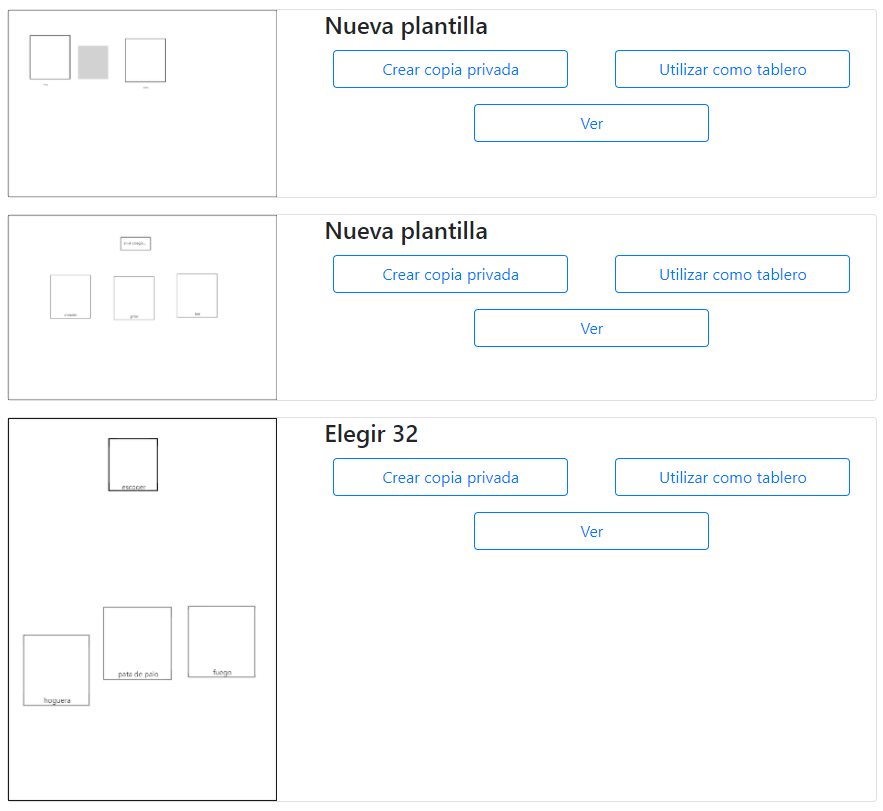
\includegraphics[width=0.7\linewidth]{Imagenes/Bitmap/PictablerosPlantilla}
		\caption{Menú de Pictableros para utilizar una plantilla pública.}
		\label{fig:pictablerosplantilla}
	\end{figure}
	
	
	\item \textbf{Tableros}: al igual que en el apartado anterior, la sección de tableros consta de tres secciones: públicos, crear nuevos y privados. En el apartado de públicos aparecen tableros ya creados que podremos duplicar como copia privada y modificarlo, o ver el tablero. En crear nuevo ofrece la posibilidad de insertar en el tablero áreas para añadir pictogramas, insertar texto y formas geométricas, se puede ver un ejemplo de creación de un tablero en la Figura \ref{fig:tableropictableros}. Por último en la sección de tableros privados podremos importar o exportar tableros que tengamos en nuestro equipo.
	
	% TODO: \usepackage{graphicx} required
	\begin{figure}[h!]
		\centering
		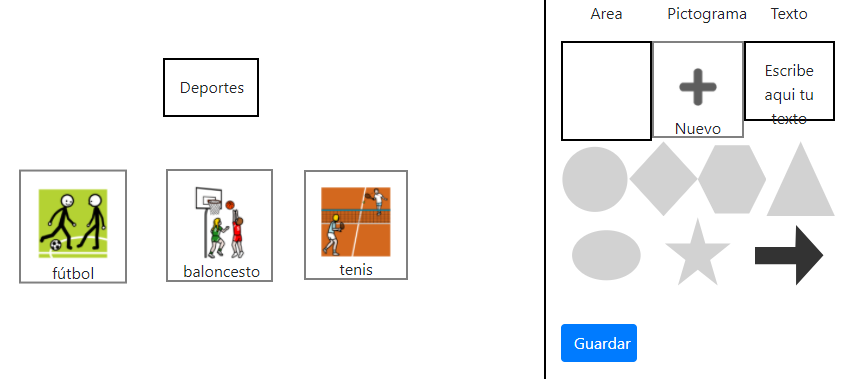
\includegraphics[width=0.7\linewidth]{Imagenes/Bitmap/tableroPicTableros}
		\caption{Ejemplo de creación de un tablero con un campo de texto y pictogramas.}
		\label{fig:tableropictableros}
	\end{figure}
	
	
\end{itemize}


	
\subsection{Symbo Talk}
\label{cap2:sec:symbotalk}
Symbo Talk\footnote{\url{  https://civat.es/app/symbo-talk/ }} permite la creación de tableros de comunicación aumentativa y locución de tableros y pictogramas mediante su aplicación web o dispositivos móviles como Android e iOS.

SymboTalk ofrece dos modos de usuario:

\begin{itemize}
	\item \textbf{Modo edición}: permite la creación de pictogramas, construir tableros y buscar pictogramas en un buscador. También ofrece la opción de crear un perfil y poder guardar todos los tableros que hayamos realizado.
	
	
	\item \textbf{Modo usuario}: pensado para que el usuario pueda comunicarse de una forma más fácil e intuitiva. Permite usar los pictogramas de la biblioteca o los que hayamos creado y reproducir por voz la secuencia de pictogramas seleccionada. En la Figura \ref{fig:symbotalk} podemos ver la pantalla principal de este modo. En el modo usuario permite editar el perfil para hacerlo lo más afín al usuario que lo utilice y que éste se sienta más cómodo a la hora de usar la aplicación.
	
	
\end{itemize}

% TODO: \usepackage{graphicx} required
\begin{figure}[h!]
	\centering
	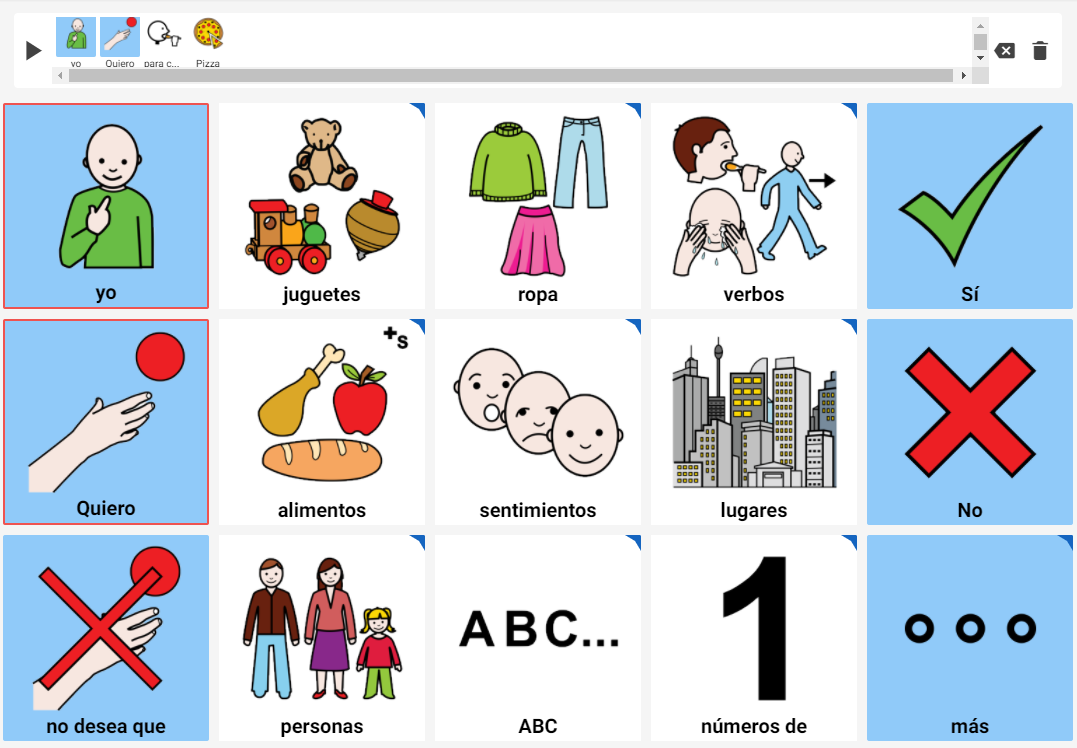
\includegraphics[width=0.7\linewidth]{Imagenes/Bitmap/SymboTalk}
	\caption{Pantalla principal de la aplicación Symbo Talk.}
	\label{fig:symbotalk}
\end{figure}

\newpage
\subsection{LetMe Talk}

LetMe Talk\footnote{\url{ https://www.letmetalk.info/es}} es una aplicación para dispositivos Android e iOS que permite generar frases a partir de una lista de  pictogramas seleccionados. Al ser descargada contiene una pequeña selección de pictogramas separadas por categorías (ver Figura \ref{fig:letmetalk}) como “General”, “Comida” o “Juguetes”. Al pulsar en cualquiera de estos pictogramas, se desplegará otro tablero donde aparecen pictogramas con juguetes como “muñeca” o “pelota”. 
Ofrece un total de 9.000 pictogramas de \textit{ARASAAC} y la posibilidad de añadir imágenes del móvil para ser incluidas como pictogramas con texto personalizado. 


% TODO: \usepackage{graphicx} required
\begin{figure}[h!]
	\centering
	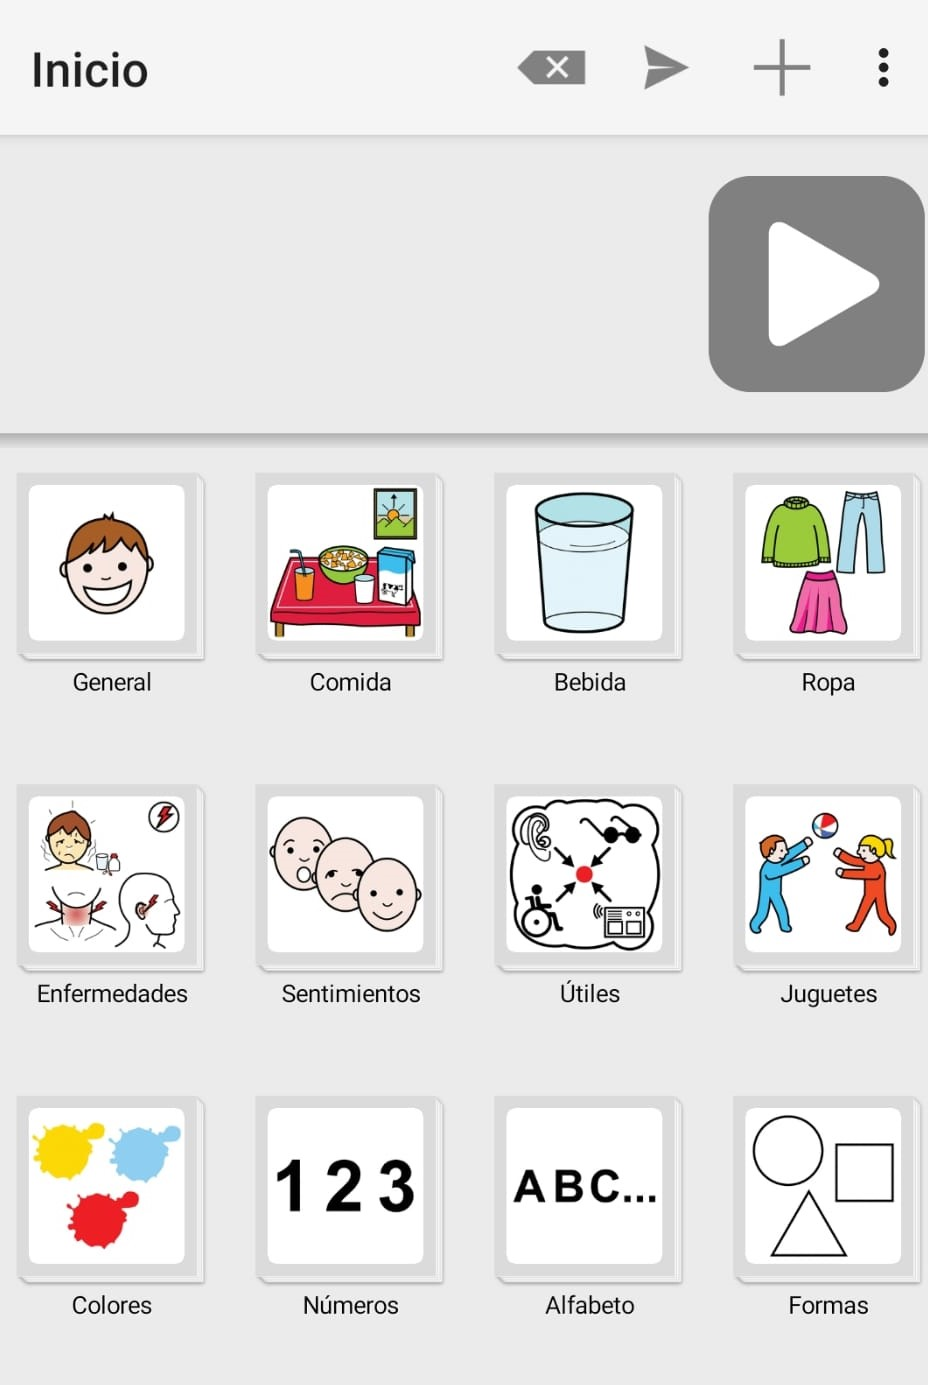
\includegraphics[width=0.7\linewidth]{Imagenes/Bitmap/LetMeTalk}
	\caption{Menú de la aplicación en Android de LetMe Talk.}
	\label{fig:letmetalk}
\end{figure}

\newpage

\subsection{Jocomunico}
\label{cap2:jocomunico}
Jocomunico\footnote{\url{http://joanpahisa.com/es/jocomunico/}} es una aplicación basada en el uso de pictogramas para ayudar a personas con dificultad en el habla. Su aplicación se puede usar tanto en su página web como en dispositivos Android e iOS y Windows y Mac OS X.

Jocomunico se creó con el objetivo de poder ayudar a los logopedas a trabajar con personas con dificultades comunicativas y poder facilitar las tareas de aprendizaje de los tiempos verbales, creación de distintos tipos de frases (preguntas, negaciones, etc) o estructurar de manera correctas los textos.

La aplicación cuenta con múltiples ajustes de accesibilidad que permiten la manera en la que se puede seleccionar un pictograma dependiendo del dispositivo ya sea de manera táctil, con uno o dos toques, o con el ratón del ordenador. También ofrece servicios de síntesis de voz para poder reproducir una secuencia de pictogramas creada por medio de los altavoces de nuestros dispositivos.

Una característica muy importante de esta aplicación es que aprende del uso que le da el usuario a los pictogramas y permite predecir pictogramas que le pueden ser útiles según está generando una frase, como se puede ver en el recuadro azul situado a la izquierda de la Figura \ref{fig:jocomunico}.

% TODO: \usepackage{graphicx} required
\begin{figure}[h!]
	\centering
	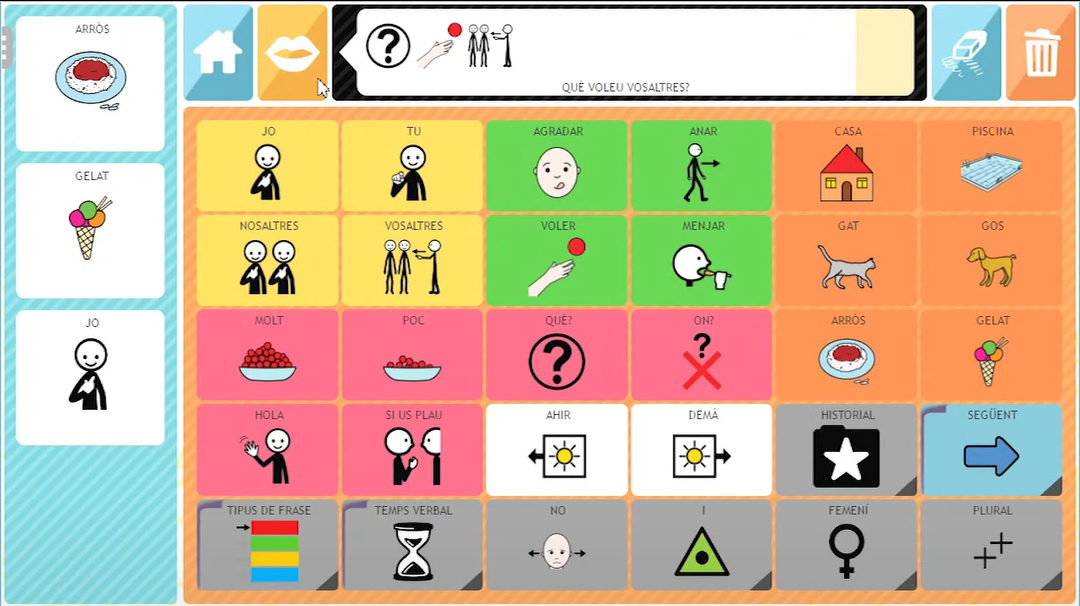
\includegraphics[width=0.7\linewidth]{Imagenes/Bitmap/jocomunico}
	\caption{Pantalla principal de la aplicación Jocomunico.}
	\label{fig:jocomunico}
\end{figure}


\section{Comparativa de las herramientas analizadas}
\label{cap2:tablacomparativa}
Tras haber analizado las aplicaciones mencionadas anteriormente se han recopilado aspectos que muchas de ellas tienen en común y funcionalidades que no tienen en la Tabla \ref{tab:comparativa}.



\begin{table}[]
	\centering
	\resizebox{13cm}{!} {
		\begin{tabular}{|l|l|l|l|l|l|l|}
			\hline
			
			\textbf{Programas} & \textbf{Disponible} & \textbf{{\begin{tabular}[c]{@{}l@{}}\\ Se mantiene \\ actualizado \\ \\\end{tabular}}} & \textbf{Dispositivos} & \textbf{{\begin{tabular}[c]{@{}l@{}}\\ Permite editar \\ pictogramas \\ \\\end{tabular}}}  & \textbf{Precio} & \textbf{{\begin{tabular}[c]{@{}l@{}}\\ Colocación de \\ pictogramas \\ \\\end{tabular}}} \\  \hline
			
			\textbf{Pictoselector} &Sí  &Sí  &PC y MAC  &Sí &Gratuito &{\begin{tabular}[c]{@{}l@{}} \\No \\ \\ \end{tabular}} \\ \hline
			\textbf{Editor ARASAAC} &Sí  &Sí  &{\begin{tabular}[c]{@{}l@{}}\\PC, MAC, Android, \\ iOS y Web \end{tabular}}  &Sí &Gratuito &{\begin{tabular}[c]{@{}l@{}} \\No \\ \\ \end{tabular}} \\ \hline
			\textbf{Piktoplus} &No  &No  &Android  &No &139€ &{\begin{tabular}[c]{@{}l@{}} \\No \\ \\ \end{tabular}}\\ \hline
			\textbf{Pictar} &Sí  &{\begin{tabular}[c]{@{}l@{}}\\La web no, \\los pictogramas sí\end{tabular}}  &Web  &No &Gratuito &{\begin{tabular}[c]{@{}l@{}} \\Sí \\ \\ \end{tabular}}\\ \hline
			\textbf{Pictableros} &Sí  &{\begin{tabular}[c]{@{}l@{}}\\La web no, \\los pictogramas sí\end{tabular}}   &Web  &Sí &Gratuito &{\begin{tabular}[c]{@{}l@{}} \\Sí \\ \\ \end{tabular}}\\ \hline
			\textbf{Jocomunico} &Sí  &Sí  &Web  &No &Gratuito &{\begin{tabular}[c]{@{}l@{}} \\No \\ \\ \end{tabular}}\\ \hline
			
			
		\end{tabular}
	}
	\caption{\label{tab:comparativa}Tabla comparativa entre los distintos editores de tableros basados en pictogramas}
\end{table}

Podemos observar que muchas de ellas se pueden descargar a través de la Play Store, App Store o utilizar su servicio desde su página web. Los más completos o que ofrecen más opciones, están disponibles para ordenadores. Aunque en dispositivos móviles hay mayor oferta  de aplicaciones, generalmente ofrecen pocas opciones o funcionalidades. Además es importante destacar que no todas las aplicaciones cuentan con bases de datos de pictogramas actualizadas.

Aunque a pesar de todo, el factor determinante es el precio. Las aplicaciones que no son gratuitas tienen un precio desorbitado que muchas familias o docentes no pueden permitirse, por ello que la aplicación sea gratuita es determinante. Respecto a los idiomas, destacan el español y el inglés como idiomas predominantes entre las distintas aplicaciones. 

Muchas de estas aplicaciones no permiten la creación de tableros en los que poder colocar los pictogramas libremente ni insertar texto o iconos, simplemente tienen una cuadrícula donde se van insertando en orden los pictogramas seleccionados por el usuario. Un aspecto muy importante que se va a desarrollar en nuestra aplicación y que muy pocas ofrecen la posibilidad es permitir que el usuario pueda cargar sus propias imágenes y utilizarlas como si fueran pictogramas, con su imagen y texto correspondiente.

Como conclusión final tras haber analizado todas las principales características de las aplicaciones mencionadas anteriormente, decidimos que se deberían tener en cuenta para el desarrollo de la aplicación las siguientes características:


\begin{itemize}
	\item La aplicación debe de ser gratuita y accesible desde el navegador web. Para ser alcanzar al mayor número de usuarios posibles.
	\item Ofrecer la posibilidad de personalizar los pictogramas para transmitir más información en un mismo picto y si el pictograma lo permite que se asemeje a los rasgos físicos del usuario que utilice los pictogramas. Ya que de esta manera, se podrá sentir identificado por un pictograma fácilmente. 
	\item La base de datos debe de contar con los últimos pictogramas creados del sistema pictográfico utilizado. 
	\item La aplicación debe permitir desplazar con libertad los pictogramas en el tablero para que los usuarios puedan crear material con el diseño que deseen. 
	\item La aplicación debe permitir al usuario subir imágenes para que sean utilizadas en el tablero. Esta característica permitirá crear nuevos tipos de materiales que se complementen con los pictogramas y otros elementos.
	\item La aplicación debe permitir añadir figuras e iconos para personalizar el diseño del tablero.
	
	
\end{itemize}





